\documentclass[12pt,a4paper]{article}
% \usepackage[latin1]{inputenc}
\usepackage[english]{babel}
\usepackage{amsmath}
\usepackage{amsfonts}
\usepackage{amssymb}
\usepackage{svg}
\usepackage{float}
\usepackage{url}
\usepackage{hyperref}

\author{
  Katrien Laenen\\
  \and
  Gust Verbruggen\\
  \and
  Ward Schodts
}
\title{Knowledge \& the web: exercise session 6}
\begin{document}
\maketitle
In this report we discuss which algorithms we tried to find a good classification model that predicts if a passenger of the Titanic will survive or not.

We use the data from \texttt{titanic\_train.csv} to train our model and perform cross-validation for performance assessment. The models used are a \textbf{rule set} and a \textbf{decision tree}.  The rest of this document is structured as follows. First we describe the preprocessing steps used in order to prepare the data for better classification. Next, we describe the learning process for both models. Finally, we compare results for both learning techniques, based on the cross-validation results. 

\section{Preprocessing}
In order to achieve better classification, we preprocess the data. This is done in two phases: feature selection to only preserve relevant features and feature engineering in the form of a discretisation step.

\paragraph{Feature selection} Features that we do not think are relevant are \texttt{Name}, \texttt{Ticket}, \texttt{PassengerId}, \texttt{Embarked} and \texttt{Cabin}. They are removed.

\paragraph{Discretisation} The two numerical values are discretised in accordance to some criterium. The \texttt{Age} feature into five age classes: child ($<$ 9 years), teen (10 to 15 years), young (15 to 24 years), adult (25 to 59 years) and elderly ($>$ 59 years). To discretise \texttt{Fare}, we take a look at a histogram plot, as seen in Figure~\ref{fig:histfare}. There are a lot more low fares. The three leftmost bars get their own bin. The chosen discretisation is: 0-10, 10-20, 20-30, 30-100 and 100+.

\begin{figure}[htbp]
	\centering
	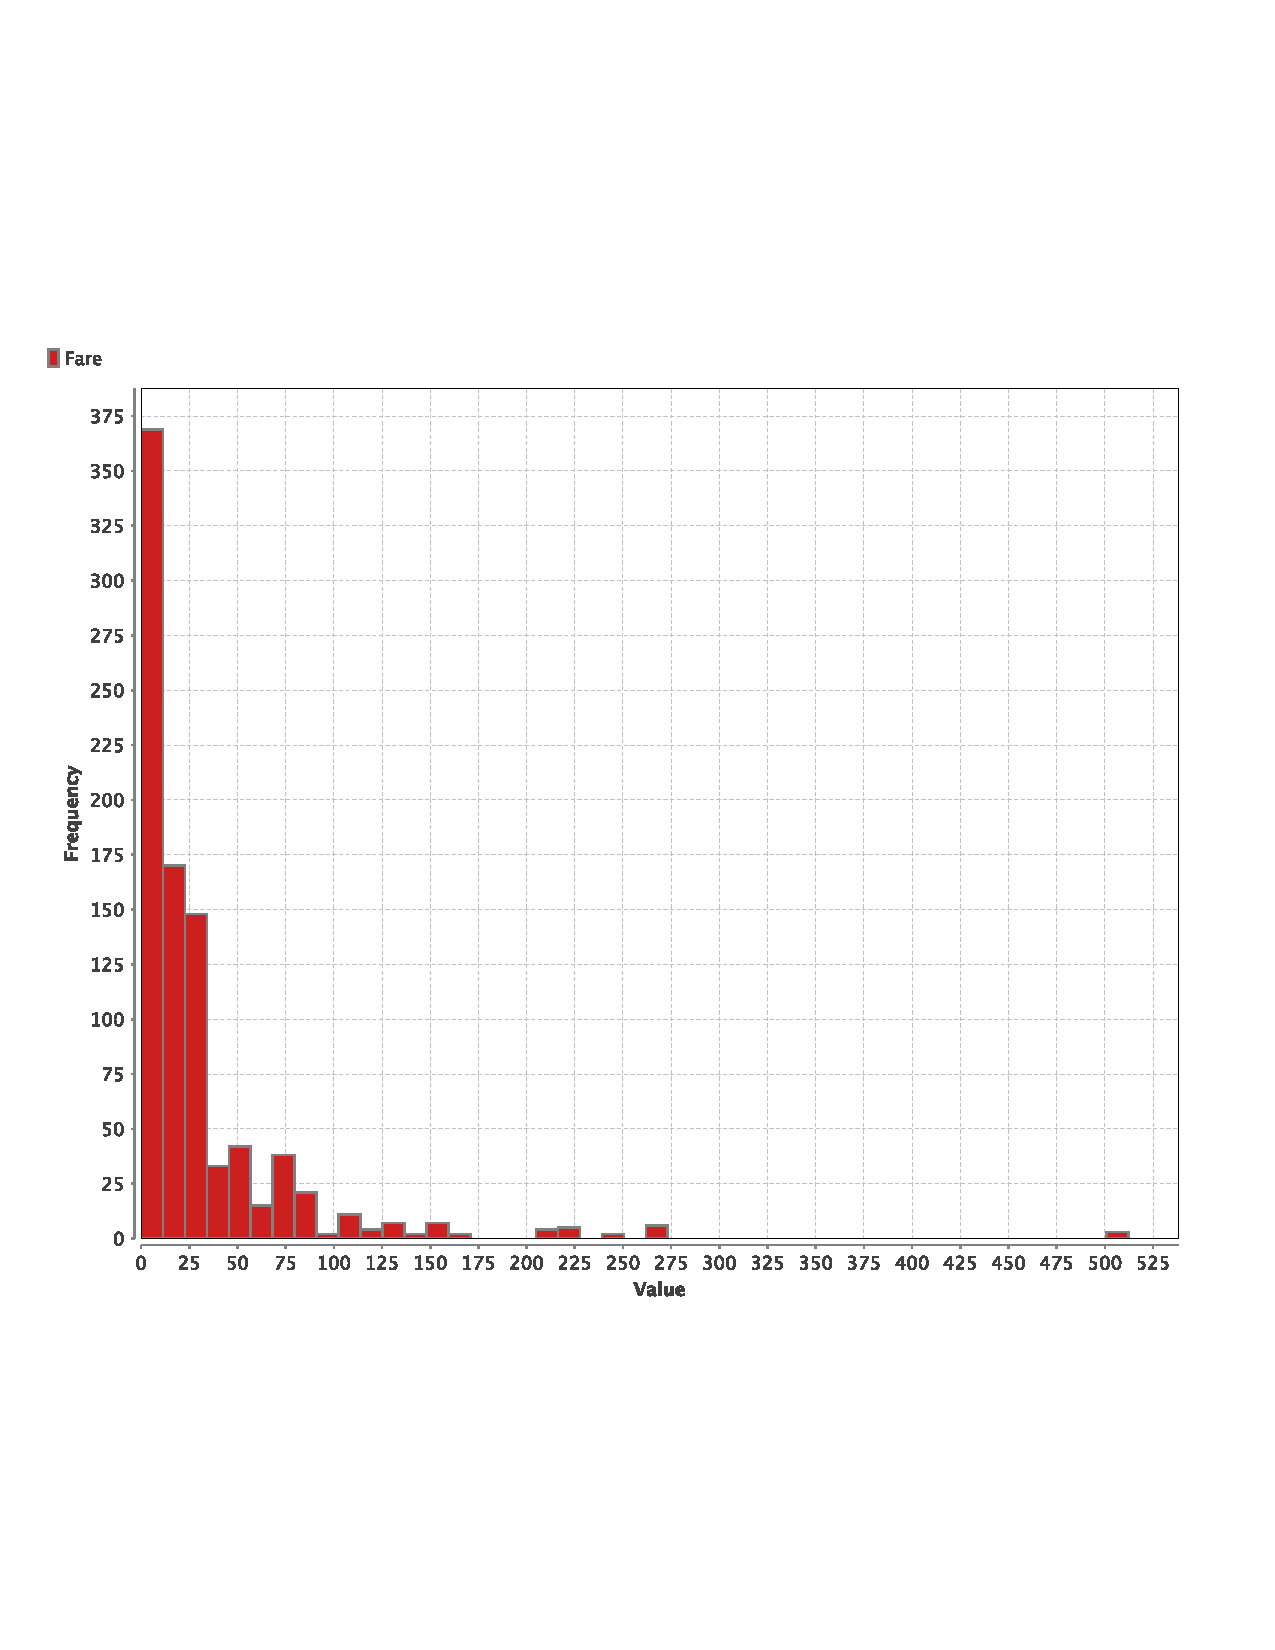
\includegraphics[width = .7\textwidth]{fare_histogram.pdf}
	\caption{Histogram for the \texttt{Fare} feature}
	\label{fig:histfare}
\end{figure}


\section{Rule learning}
One model we tried was to learn classification rules from the training data. Rule learning algorithms come with different options for several aspects of the algorithms. In the exercise session we experimented with two of these.
\par First, for choosing the conditions of a classification rule, there are two options: one is to add to the rule the condition which increases the accuracy the most, another is to add to the rule the condition which increases the information gain the most. The first option resulted in a rule set consisting of 363 rules which clearly overfitted the training data.
The second option resulted in this rule set:
\begin{itemize}

\item if Sex = male and Fare $\leq$ 15.173 then 0  (268 / 35)
\item if Sex = female and Fare $\textgreater$ 48.200 then 1  (4 / 76)
\item if Sex = male and Cabin = ? then 0  (0 / 0)
\item if Sex = male then 0  (152 / 62)
\item else 1  (61 / 121)

\end{itemize}
which is correct for 617 out of 779 training examples.
When evaluated on the test set, we got an accuracy of ?\\
A second aspect of rule learning is the desired pureness, which is the minimum ratio of the major class in a covered subset in order to consider the subset pure. The standard value for this is 0.9. We experimented with this value set to 0.8 and 1.
For the desired pureness set to 0.8 and the information criterion we got the following rule set:
\begin{itemize}

\item if Sex = male then 0  (420 / 97)
\item else 1  (64 / 189)

\end{itemize}
which is correct for 609 out of 770 training examples.
When evaluated on the test set, we got an accuracy of ?.
For the desired pureness set to 1 and the information gain criterion we got the following rule set:
\begin{itemize}

\item if Sex = male and Fare $\leq$ 15.173 then 0  (268 / 35)
\item if Sex = female and Fare $\textgreater$ 48.200 then 1  (4 / 76)
\item if Sex = male and Cabin = ? then 0  (0 / 0)
\item if Sex = male then 0  (152 / 62)
\item else 1  (61 / 121)

\end{itemize}
which is the same as the first rule set, which was obtained with the standard value for the desired pureness.\\
Next to these two, there are three other parameters for rule learning: sample ratio (which specifies the sample ratio of training data used for growing and pruning), minimal prune benefit (which specifies the minimum amount of benefit which must be exceeded over unpruned benefit in order to be pruned) and use local random seed (which indicates if a local random seed should be used for randomization). We did not experiment with these parameters, but kept the standard values for these, which were 0.9, 0.25 and no respectively.\\
\\
From these results we can clearly see that Sex, Fare and SibSp are features which are important for this task. That Sex and Fare were important features was to be expected. When the Titanic collided with an iceberg, women and children and people of the higher ranks were evacuated first. This is reflected in the data as we see that women and people which payed a higher fare are more likely to have survived. That the number of siblings and spouses is also an important feature can be explained as follows. People in need want to stay close to their loved ones at all costs. But how larger a group, how more difficult it was to get on a lifeboat together. As such, how more siblings and spouses someone had aboard, how less likely that person was to survive.

\section{Decision trees}

Apart from \emph{rule learning} we also experimented witch decision trees. First we applied the standard decision tree in RapidMiner, it created a too complicated decision tree, as you can see in figure 1.
\begin{figure}[H]
  \centering
  \includesvg[width = 1.5\textwidth]{decisiontreetitanic_original}
  \caption{Original decision tree with maximal depth of 20}
\end{figure}
Next we limited the maximal depth of the decision tree to 3. This gave us figure 2, which is much more usefull.
\begin{figure}[H]
  \centering
  \includesvg[width = 1\textwidth]{decisiontreetitanic}
  \caption{Decision tree with maximal depth of 3}
\end{figure}


\section{Rule learning vs. Decision trees}
\begin{figure}[H]
\centering
\begin{tabular}{|c|c|c|}
\hline 
• & Precision & Accuracy \\ 
\hline 
Rule learning 1 & • & • \\ 
\hline 
Rule learning 2 & • & • \\ 
\hline 
Decision tree 1 & • & • \\ 
\hline 
Decision tree 2 & • & • \\ 
\hline 
\end{tabular} 
\caption{Overview}
\end{figure}

\end{document}
